\documentclass[letterpaper,12pt]{article}

\usepackage{threeparttable}
\usepackage{geometry}
\geometry{letterpaper,tmargin=1in,bmargin=1in,lmargin=1.25in,rmargin=1.25in}
\usepackage[format=hang,font=normalsize,labelfont=bf]{caption}
\usepackage{amsmath}
\usepackage{multirow}
\usepackage{array}
\usepackage{delarray}
\usepackage{amssymb}
\usepackage{amsthm}
\usepackage{lscape}
\usepackage{natbib}
\usepackage{setspace}
\usepackage{float,color}
\usepackage[pdftex]{graphicx}
\usepackage{pdfsync}
\usepackage{verbatim}
\usepackage{placeins}
\usepackage{geometry}
\usepackage{pdflscape}
\synctex=1
\usepackage{hyperref}
\hypersetup{colorlinks,linkcolor=red,urlcolor=blue,citecolor=red}
\usepackage{bm}
\theoremstyle{definition}
\newtheorem{theorem}{Theorem}
\newtheorem{acknowledgement}[theorem]{Acknowledgement}
\newtheorem{algorithm}[theorem]{Algorithm}
\newtheorem{axiom}[theorem]{Axiom}
\newtheorem{case}[theorem]{Case}
\newtheorem{claim}[theorem]{Claim}
\newtheorem{conclusion}[theorem]{Conclusion}
\newtheorem{condition}[theorem]{Condition}
\newtheorem{conjecture}[theorem]{Conjecture}
\newtheorem{corollary}[theorem]{Corollary}
\newtheorem{criterion}[theorem]{Criterion}
\newtheorem{definition}{Definition} % Number definitions on their own
\newtheorem{derivation}{Derivation} % Number derivations on their own
\newtheorem{example}[theorem]{Example}
\newtheorem{exercise}[theorem]{Exercise}
\newtheorem{lemma}[theorem]{Lemma}
\newtheorem{notation}[theorem]{Notation}
\newtheorem{problem}[theorem]{Problem}
\newtheorem{proposition}{Proposition} % Number propositions on their own
\newtheorem{remark}[theorem]{Remark}
\newtheorem{solution}[theorem]{Solution}
\newtheorem{summary}[theorem]{Summary}
\bibliographystyle{aer}
\newcommand\ve{\varepsilon}
\renewcommand\theenumi{\roman{enumi}}
\newcommand\norm[1]{\left\lVert#1\right\rVert}
\begin{document}
\subsection*{11.1}



Consider
 \[\hat{X}+\hat{Y}=\{\hat{X}_1+\hat{Y}_1,...,\hat{X}_T+\hat{Y}_T\}\]
\[S_{X+Y}(w)=\lim_{T \rightarrow \infty}E\{|(\hat{X+Y})^T(w)|^2\}\]
\[=\lim_{T \rightarrow \infty}E\{|(\hat{X}^T(w)+\hat{Y}^T(w))|^2\}\]
\[=\lim_{T \rightarrow \infty}E\{|((\hat{X})^T(w))^2+((\hat{Y})^T(w))^2+2\hat{X}^T(w)\hat{Y}^T(w)|\}\]
\[\le \lim_{T \rightarrow \infty}E\{|((\hat{X})^T(w))^2|\}+\lim_{T \rightarrow \infty}E\{|((\hat{Y})^T(w))^2|\}+\lim_{T \rightarrow \infty}E\{|2\hat{X}^T(w)\hat{Y}^T(w)|\}\]
\[S_{X+Y}(w)=S_X(w)+S_Y(w)+2Re(S_{XY}(w))\]

\subsection*{11.2}

By attempting to minimize left side of the equation, we have the first order conditions
\[g_1:-2(y_1-g_1)+2\lambda(g_2-2g_1+g_0)(-2)=0\]
\[-2y_1+2g_1-4\lambda(g_2-2g_1-g_0)=0\]
We also have the second order conditions
\[g2: -2(y_2-g_2)-4\lambda(g_3-2g_2+g_1)-4\lambda(g_2-2g_1+g_0)=0\]
\[-2(y_2)+2(g_2)-4 \lambda (g_3-g_2-g_1+g_0)=0\]
and thereby we have the $n^{th}$ order condition:
\[g_n:-2(y_n-g_n)^2+\lambda(2(g_{n+2}-2g_{n+1}+g_n)-4(g_{n+1}-2g_n+g_{n-1})+2(g_n-2g_{n-1}+g_{n-2}))=0\]
which yields the linear
\[-2y_n+2g_n+2\lambda(g_{n+2}-4g_{n+1}+6g_n-4g_{n-1}+g_{n-2})=0\]
\subsection*{11.3}


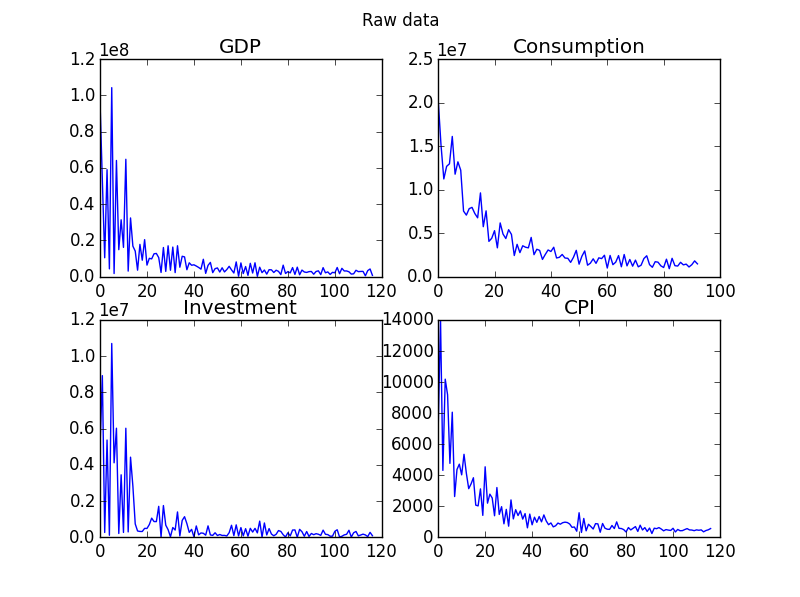
\includegraphics[scale = .75]{eleventhree}

\subsection*{11.4}


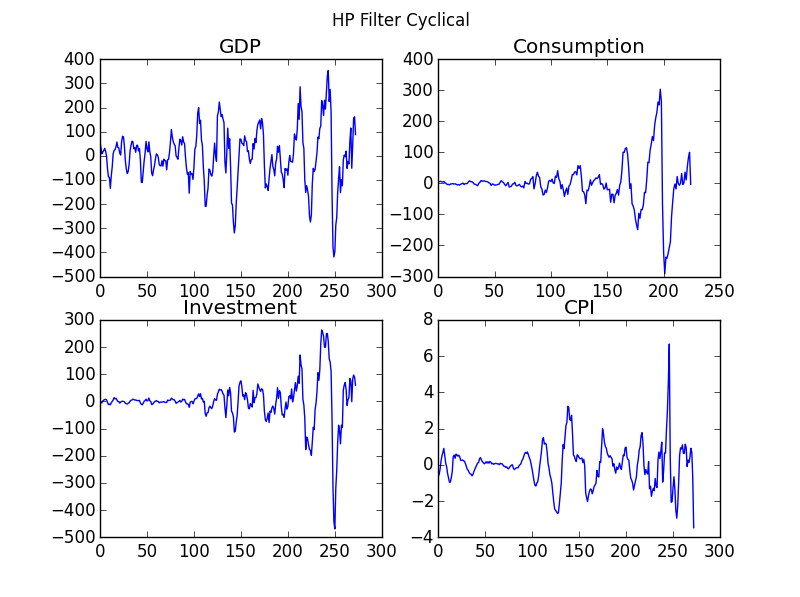
\includegraphics[scale = .75]{elevenfour}\\
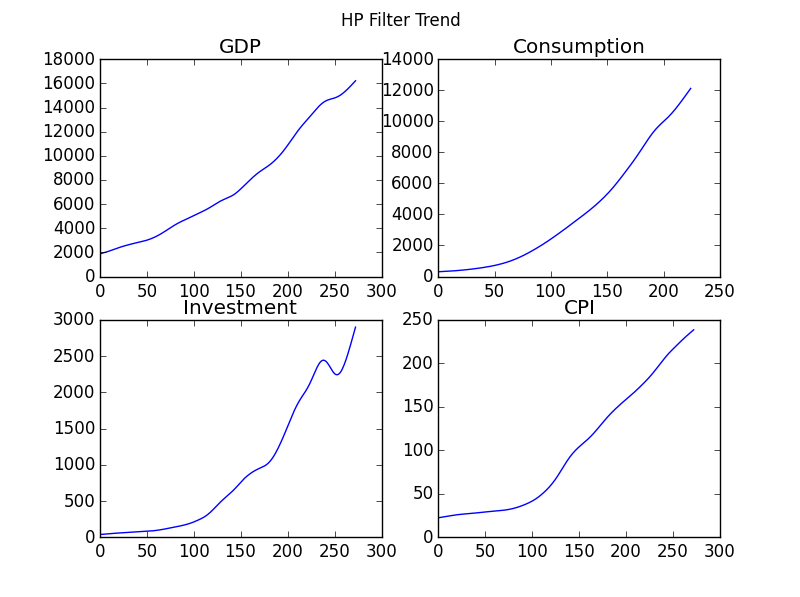
\includegraphics[scale = .75]{elvenfourhpfilter}



\subsection*{11.5}


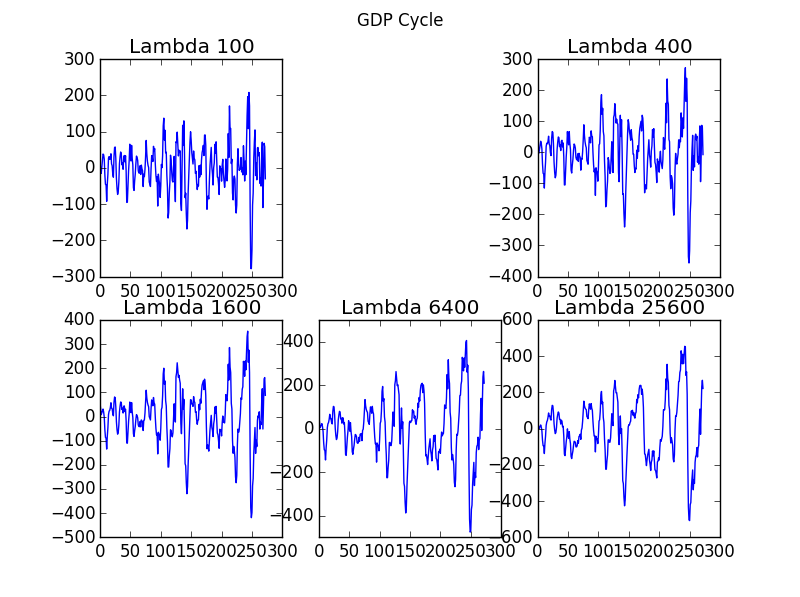
\includegraphics[scale = .75]{elevenfive}

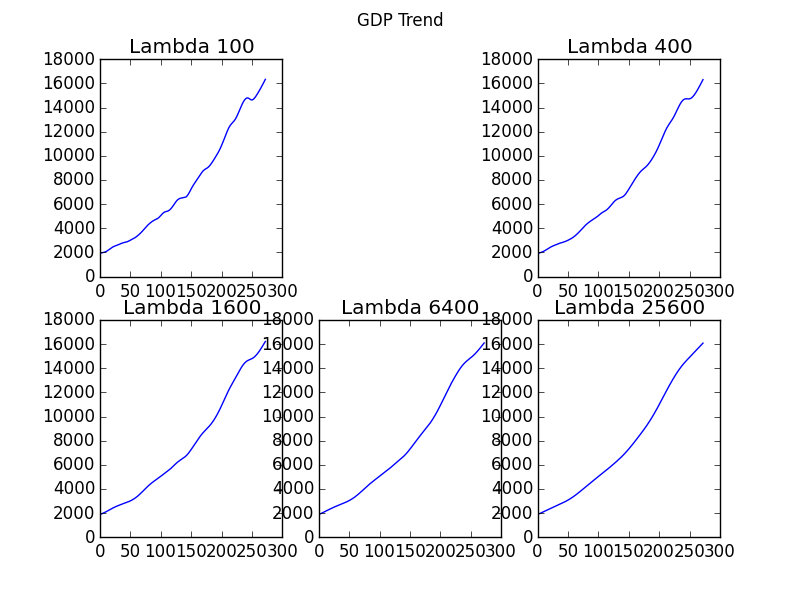
\includegraphics[scale = .75]{elevenfivesmooth}

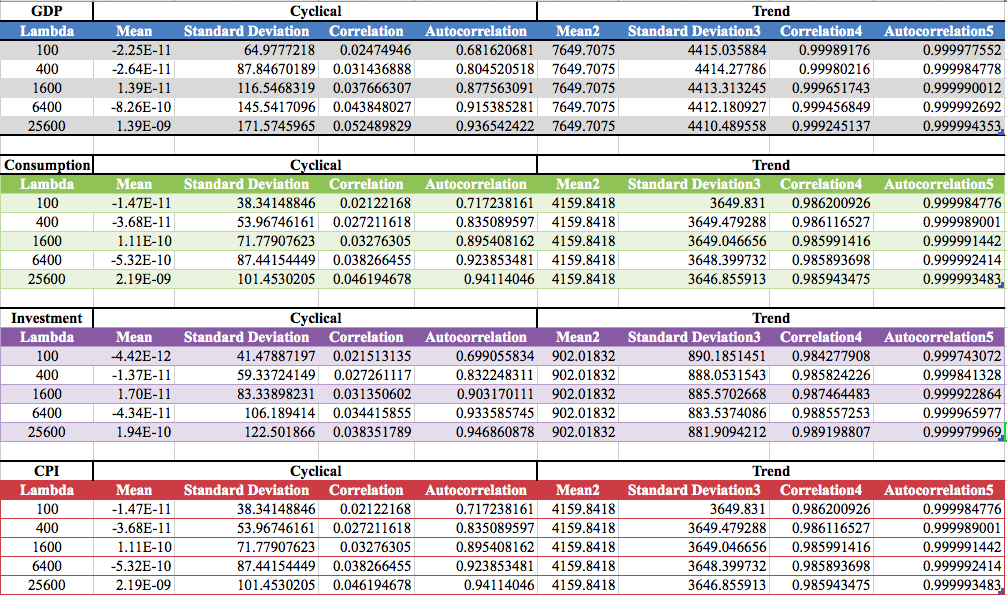
\includegraphics[scale = .50]{elevenc}

\subsection*{11.6}


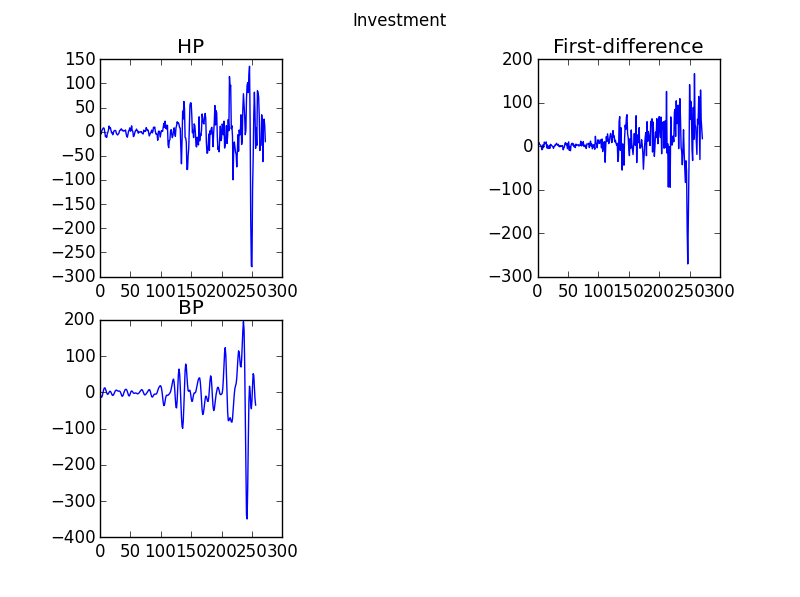
\includegraphics[scale = .75]{elevensixinvestment}

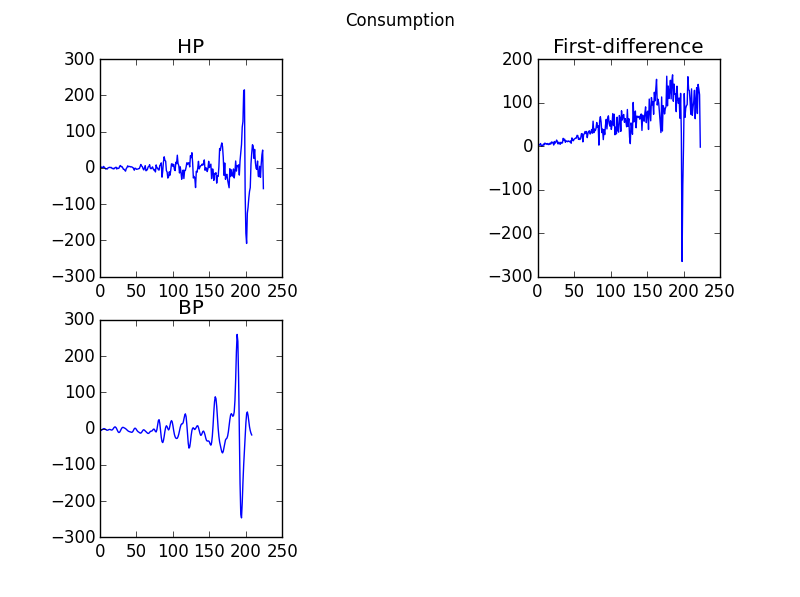
\includegraphics[scale = .75]{elevensixhp}

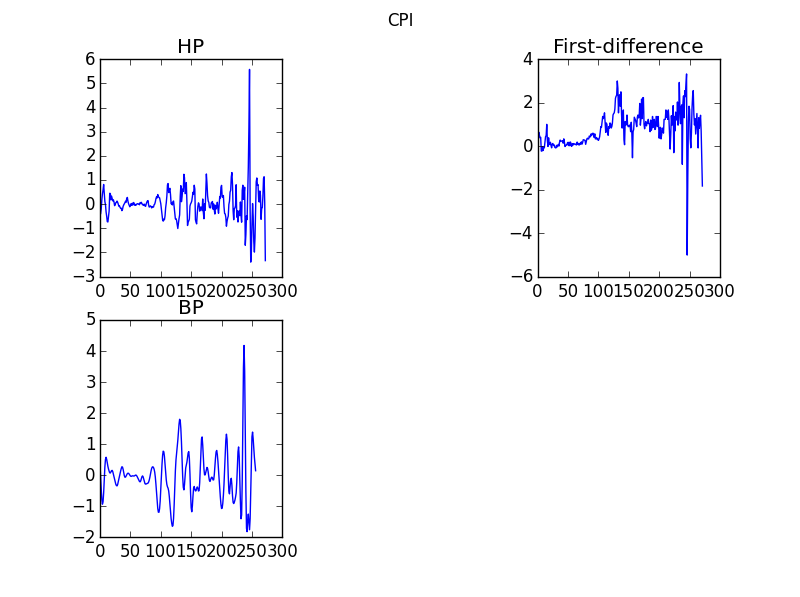
\includegraphics[scale = .75]{elevensixcpi}

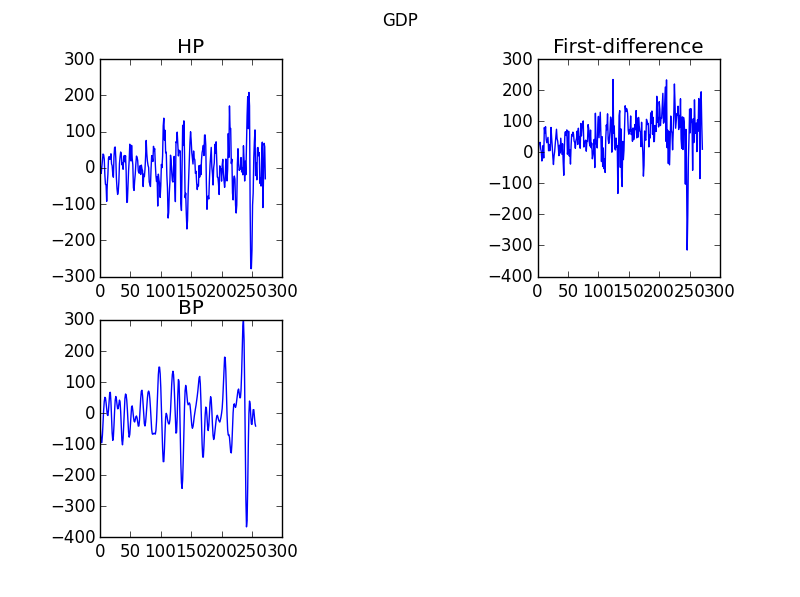
\includegraphics[scale = .75]{elevensixconsumption}
Here are the different values requested for each series:\\

GDP:\\

First-difference\\
Mean = 0.784930147059\\
Std = 0.831049857977\\
Correlation = 0.384323520588\\
Autocorrelation = 0.54495746495\\
\\
HP\\
Mean = 3.35184871311e-12\\
Std = 1.13268427423\\
Correlation = -0.00469118734317\\
Autocorrelation = 0.836207709801\\

BP\\
Mean = -0.0299699997469\\
Std = 0.780953878382\\
Correlation = 0.0518286280981\\
Autocorrelation = 0.892077087025\\
\\
Consumption:\\

First-difference\\
Mean = 52.7147321429\\
Std = 48.1384249078\\
Correlation = 0.663184463727\\
Autocorrelation = 0.689913577226\\

HP\\
Mean = 1.75837464247e-11\\
Std = 83.3389823065\\
Correlation = 0.0313506020433\\
Autocorrelation = 0.903170110974\\
\\
BP\\
Mean = -4.18832038676\\
Std = 50.9369790265\\
Correlation = -0.00499167776043\\
Autocorrelation = 0.906662966667\\
\\
Investment:\\

First-difference\\
Mean = 10.7522058824\\
Std = 41.2467110398\\
Correlation = 0.181971196678\\
Autocorrelation = 0.455339024967\\
\\
HP\\
Mean = 1.02860819122e-10\\
Std = 71.779076232\\
Correlation = 0.0327630499623\\
Autocorrelation = 0.895408162229\\
\\
BP\\
Mean = -1.64783219425\\
Std = 55.6126386658\\
Correlation = -0.0275753430097\\
Autocorrelation = 0.895068261543\\
\\
CPI:\\
\\
First-difference\\
Mean = 0.784930147059\\
Std = 0.831049857977\\
Correlation = 0.384323520588\\
Autocorrelation = 0.54495746495\\
\\
HP\\
Mean = 3.35184871311e-12\\
Std = 1.13268427423\\
Correlation = -0.00469118734317\\
Autocorrelation = 0.836207709801\\
\\
BP\\
Mean = -0.0299699997469\\
Std = 0.780953878382\\
Correlation = 0.0518286280981\\
Autocorrelation = 0.892077087025\\
\\
\subsection*{11.7}
S\&P Index:\\
\\
OLS\\
Mean = 7.20602060925\\
Std = 0.115802246374\\
Autocorrelation = 1.0\\
\\
HP\\
Mean = 3.24617825498e-13\\
Std = 0.115746507918\\
Autocorrelation = 0.806375713294\\
\\
BP\\
Mean = -0.0181075102815\\
Std = 0.121154250719\\
Autocorrelation = 0.874542562966\\
\\
First-difference\\
Mean = 0.0137429626107\\
Std = 0.0758607763258\\
Autocorrelation = 0.419822311381\\




\end{document}
